\section*{Results}

The tables below summarize within-learner trajectories rather than a strict leaderboard between base learners,
because the calibrated first-neuron widths are similar but not identical across models.

\begin{table}[ht]
\centering
\small
\setlength{\tabcolsep}{3.5pt}
\begin{tabular}{llrr@{\hspace{1.8em}}rr@{\hspace{1.8em}}r}
\toprule
Model & Regime & \multicolumn{2}{c@{\hspace{1.8em}}}{$n=1$} & \multicolumn{2}{c@{\hspace{1.8em}}}{Best $n$} & Built \\
\cmidrule(lr){3-4}\cmidrule(lr){5-6}
 & & Features & Accuracy & $n$ & Accuracy & neurons \\
\midrule
\texttt{cpl} & $C_{\mathrm{low}}$ & 4.43 & 0.7690 & 4 & 0.7710 & 13 \\
\texttt{svm} & $C_{\mathrm{low}}$ & 5.73 & 0.8538 & 3 & 0.8545 & 30 \\
\texttt{logreg} & $C_{\mathrm{low}}$ & 3.82 & 0.8524 & 1 & 0.8524 & 3 \\
\midrule
\texttt{cpl} & $C_{\mathrm{high}}$ & 23.42 & 0.8245 & 4 & 0.8493 & 31 \\
\texttt{svm} & $C_{\mathrm{high}}$ & 21.54 & 0.8326 & 3 & 0.8514 & 31 \\
\texttt{logreg} & $C_{\mathrm{high}}$ & 23.89 & 0.8667 & 1 & 0.8667 & 8 \\
\bottomrule
\end{tabular}
\caption{Summary of the repeated-CV results on the colon cancer benchmark. The table reports the average width and
mean vote accuracy of the first neuron, the neuron depth at which the best mean vote accuracy was achieved,
the corresponding mean accuracy, and the realized number of neurons.}
\label{tab:colon_summary}
\end{table}

\subsection*{Colon cancer benchmark}
On the colon cancer benchmark, the low-feature regime showed learner-specific behavior across the first few
successive neurons.
For \texttt{cpl} with $C_{\mathrm{low}}$, the mean vote accuracy increased from 0.7690 for the first neuron to
0.7710 at $n=4$, while the average first-neuron width was 4.43 features.
For \texttt{svm} with $C_{\mathrm{low}}$, accuracy increased slightly from 0.8538 at $n=1$ to 0.8545 at $n=3$.
For \texttt{logreg} with $C_{\mathrm{low}}$, the best mean vote accuracy was already obtained by the first neuron
(0.8524), and only three neurons were built before the feature space was exhausted under this setting.

The high-feature regime produced a different pattern.
For \texttt{cpl} with $C_{\mathrm{high}}$, the mean vote accuracy improved from 0.8245 at $n=1$ to 0.8493 at
$n=4$.
For \texttt{svm} with $C_{\mathrm{high}}$, accuracy increased from 0.8326 at $n=1$ to 0.8514 at $n=3$.
In contrast, \texttt{logreg} with $C_{\mathrm{high}}$ achieved the highest colon cancer accuracy in this
evaluation at the first neuron (0.8667), and additional neurons did not improve the vote.

The weighted vote based on training-fold balanced accuracy did not materially change the qualitative pattern of
the colon cancer results. It matched the best unweighted result for low-feature \texttt{svm}
(0.8545 at $n=3$), low-feature \texttt{logreg} (0.8524 at $n=1$), high-feature \texttt{svm} (0.8514 at $n=3$),
and high-feature \texttt{logreg} (0.8667 at $n=1$).
For \texttt{cpl}, the weighted vote was very close to the unweighted vote, reaching 0.7698 at $n=4$ in the
low-feature regime and 0.8481 at $n=4$ in the high-feature regime.

Taken together, the colon cancer results indicate that useful complementary signal often appears in
the first few neurons, but the benefit of depth depends strongly on the base learner and feature-count regime.
The trajectory figures therefore focus on the low-feature regime, where neuron depth is most informative and
successive neurons have the clearest opportunity to add complementary signal. High-feature regimes are summarized
in Table~\ref{tab:colon_summary} and discussed in the text as a contrasting case.

\begin{figure}[!htbp]
\centering
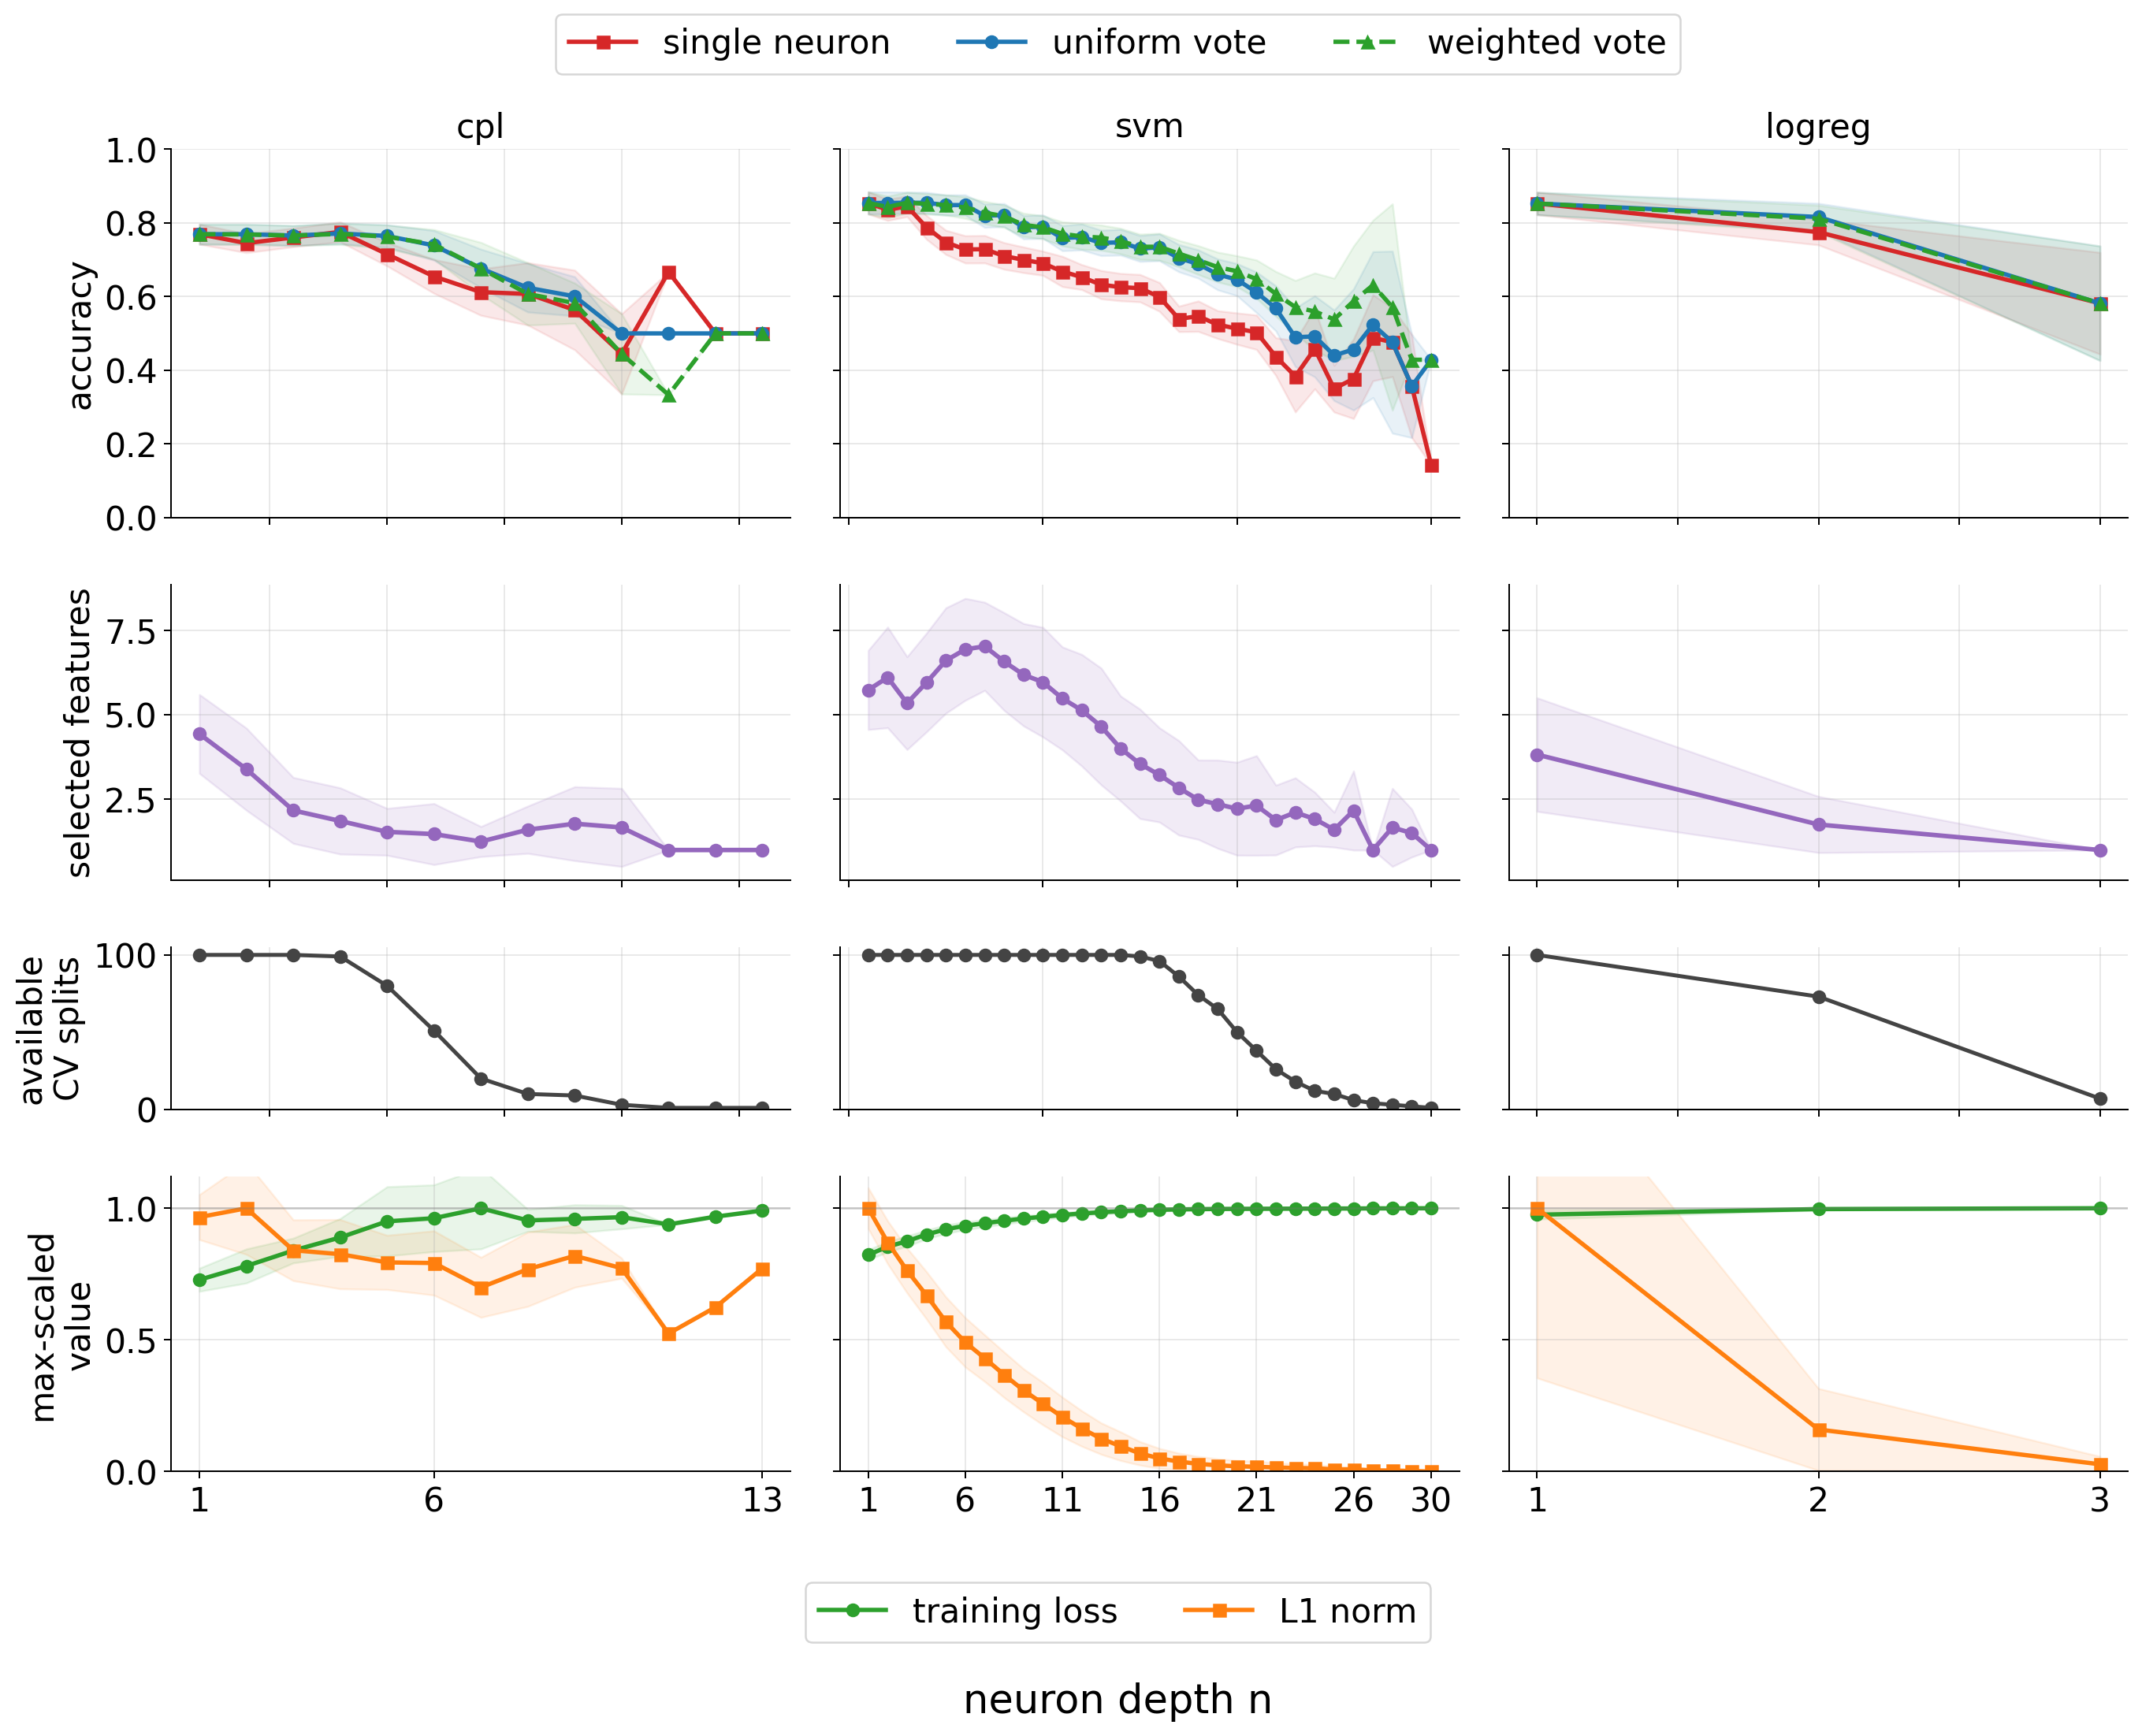
\includegraphics[width=\linewidth]{figures/paper_panels/colon_diagnostics_panel.png}
\caption{Low-feature diagnostic trajectories on the colon cancer benchmark. Columns show \texttt{cpl},
\texttt{svm}, and \texttt{logreg} with $C_{\mathrm{low}}$. Rows report predictive accuracy, the average number
of features selected by the $n$-th neuron, the number of CV splits in which that neuron depth was available,
and optimization diagnostics for the $n$-th neuron. Training loss and L1 norm are divided by their
within-model maximum values and should be interpreted as shape summaries rather than absolute-scale comparisons.}
\label{fig:colon_sparse_accuracy}
\end{figure}

\FloatBarrier

\subsection*{Synthetic predictive performance}
The synthetic benchmark first mirrors the colon cancer evaluation by comparing predictive trajectories across
learners and feature-count regimes. Its known ground truth is used separately below to analyze feature recovery.

\begin{table}[ht]
\centering
\small
\setlength{\tabcolsep}{3.5pt}
\begin{tabular}{llrr@{\hspace{1.8em}}rr@{\hspace{1.8em}}r}
\toprule
Model & Regime & \multicolumn{2}{c@{\hspace{1.8em}}}{$n=1$} & \multicolumn{2}{c@{\hspace{1.8em}}}{Best $n$} & Built \\
\cmidrule(lr){3-4}\cmidrule(lr){5-6}
 & & Features & Accuracy & $n$ & Accuracy & neurons \\
\midrule
\texttt{cpl} & $C_{\mathrm{low}}$ & 5.03 & 0.8180 & 3 & 0.8430 & 8 \\
\texttt{svm} & $C_{\mathrm{low}}$ & 6.42 & 0.8250 & 3 & 0.8500 & 8 \\
\texttt{logreg} & $C_{\mathrm{low}}$ & 3.44 & 0.6950 & 2 & 0.7424 & 3 \\
\midrule
\texttt{cpl} & $C_{\mathrm{high}}$ & 25.94 & 0.8160 & 3 & 0.8480 & 10 \\
\texttt{svm} & $C_{\mathrm{high}}$ & 25.32 & 0.8400 & 4 & 0.8490 & 13 \\
\texttt{logreg} & $C_{\mathrm{high}}$ & 27.58 & 0.8590 & 1 & 0.8590 & 7 \\
\bottomrule
\end{tabular}
\caption{Summary of the repeated-CV predictive results on the synthetic benchmark. The table follows the same
format as Table~\ref{tab:colon_summary}, reporting first-neuron width and accuracy, the best mean vote accuracy
and its depth, and the realized number of neurons.}
\label{tab:synthetic_performance}
\end{table}

In the low-feature regime, later neurons frequently improved predictive performance.
For \texttt{cpl} with $C_{\mathrm{low}}$, accuracy increased from 0.8180 at $n=1$ to 0.8430 at $n=3$, while
the first neuron selected 5.03 features on average.
For \texttt{svm} with $C_{\mathrm{low}}$, the best mean vote accuracy was 0.8500 at $n=3$, compared with 0.8250 at
$n=1$.
The first neuron selected 6.42 features on average.
For \texttt{logreg} with $C_{\mathrm{low}}$, the best result occurred at $n=2$, improving from 0.6950 at $n=1$ to
0.7424 at $n=2$.

In the high-feature regime, the first neuron often captured a larger fraction of the true signal, but additional
neurons contributed less useful information.
This was clearest for \texttt{logreg} with $C_{\mathrm{high}}$, where the first neuron already achieved the best mean
accuracy of 0.8590 and selected 27.58 features on average.
For \texttt{svm} with $C_{\mathrm{high}}$, the best mean accuracy was 0.8490 at $n=4$.
For \texttt{cpl} with $C_{\mathrm{high}}$, the best mean accuracy was 0.8480 at $n=3$.

Weighted voting again gave a more nuanced picture than a uniform improvement.
When only depths available in all 100 cross-validation splits were considered, the weighted vote reached the
same best accuracy as the unweighted vote for high-feature \texttt{logreg} (0.8590 at $n=1$), and a very similar
value for high-feature \texttt{svm} (0.8420 at $n=3$ versus an unweighted best of 0.8490 at $n=4$).
It did not improve the best accuracy of low-feature \texttt{cpl} or low-feature \texttt{svm}.
The clearest weighted-vote gain appeared for low-feature \texttt{logreg}, where the
weighted vote reached 0.7678 at $n=2$ compared with the unweighted value of 0.7424.

As for the colon cancer benchmark, the trajectory figures focus on the low-feature regime, where successive
neurons are most diagnostic of how predictive performance changes across depth. High-feature behavior is reported
in Table~\ref{tab:synthetic_performance} and in the text above.

\begin{figure}[!htbp]
\centering
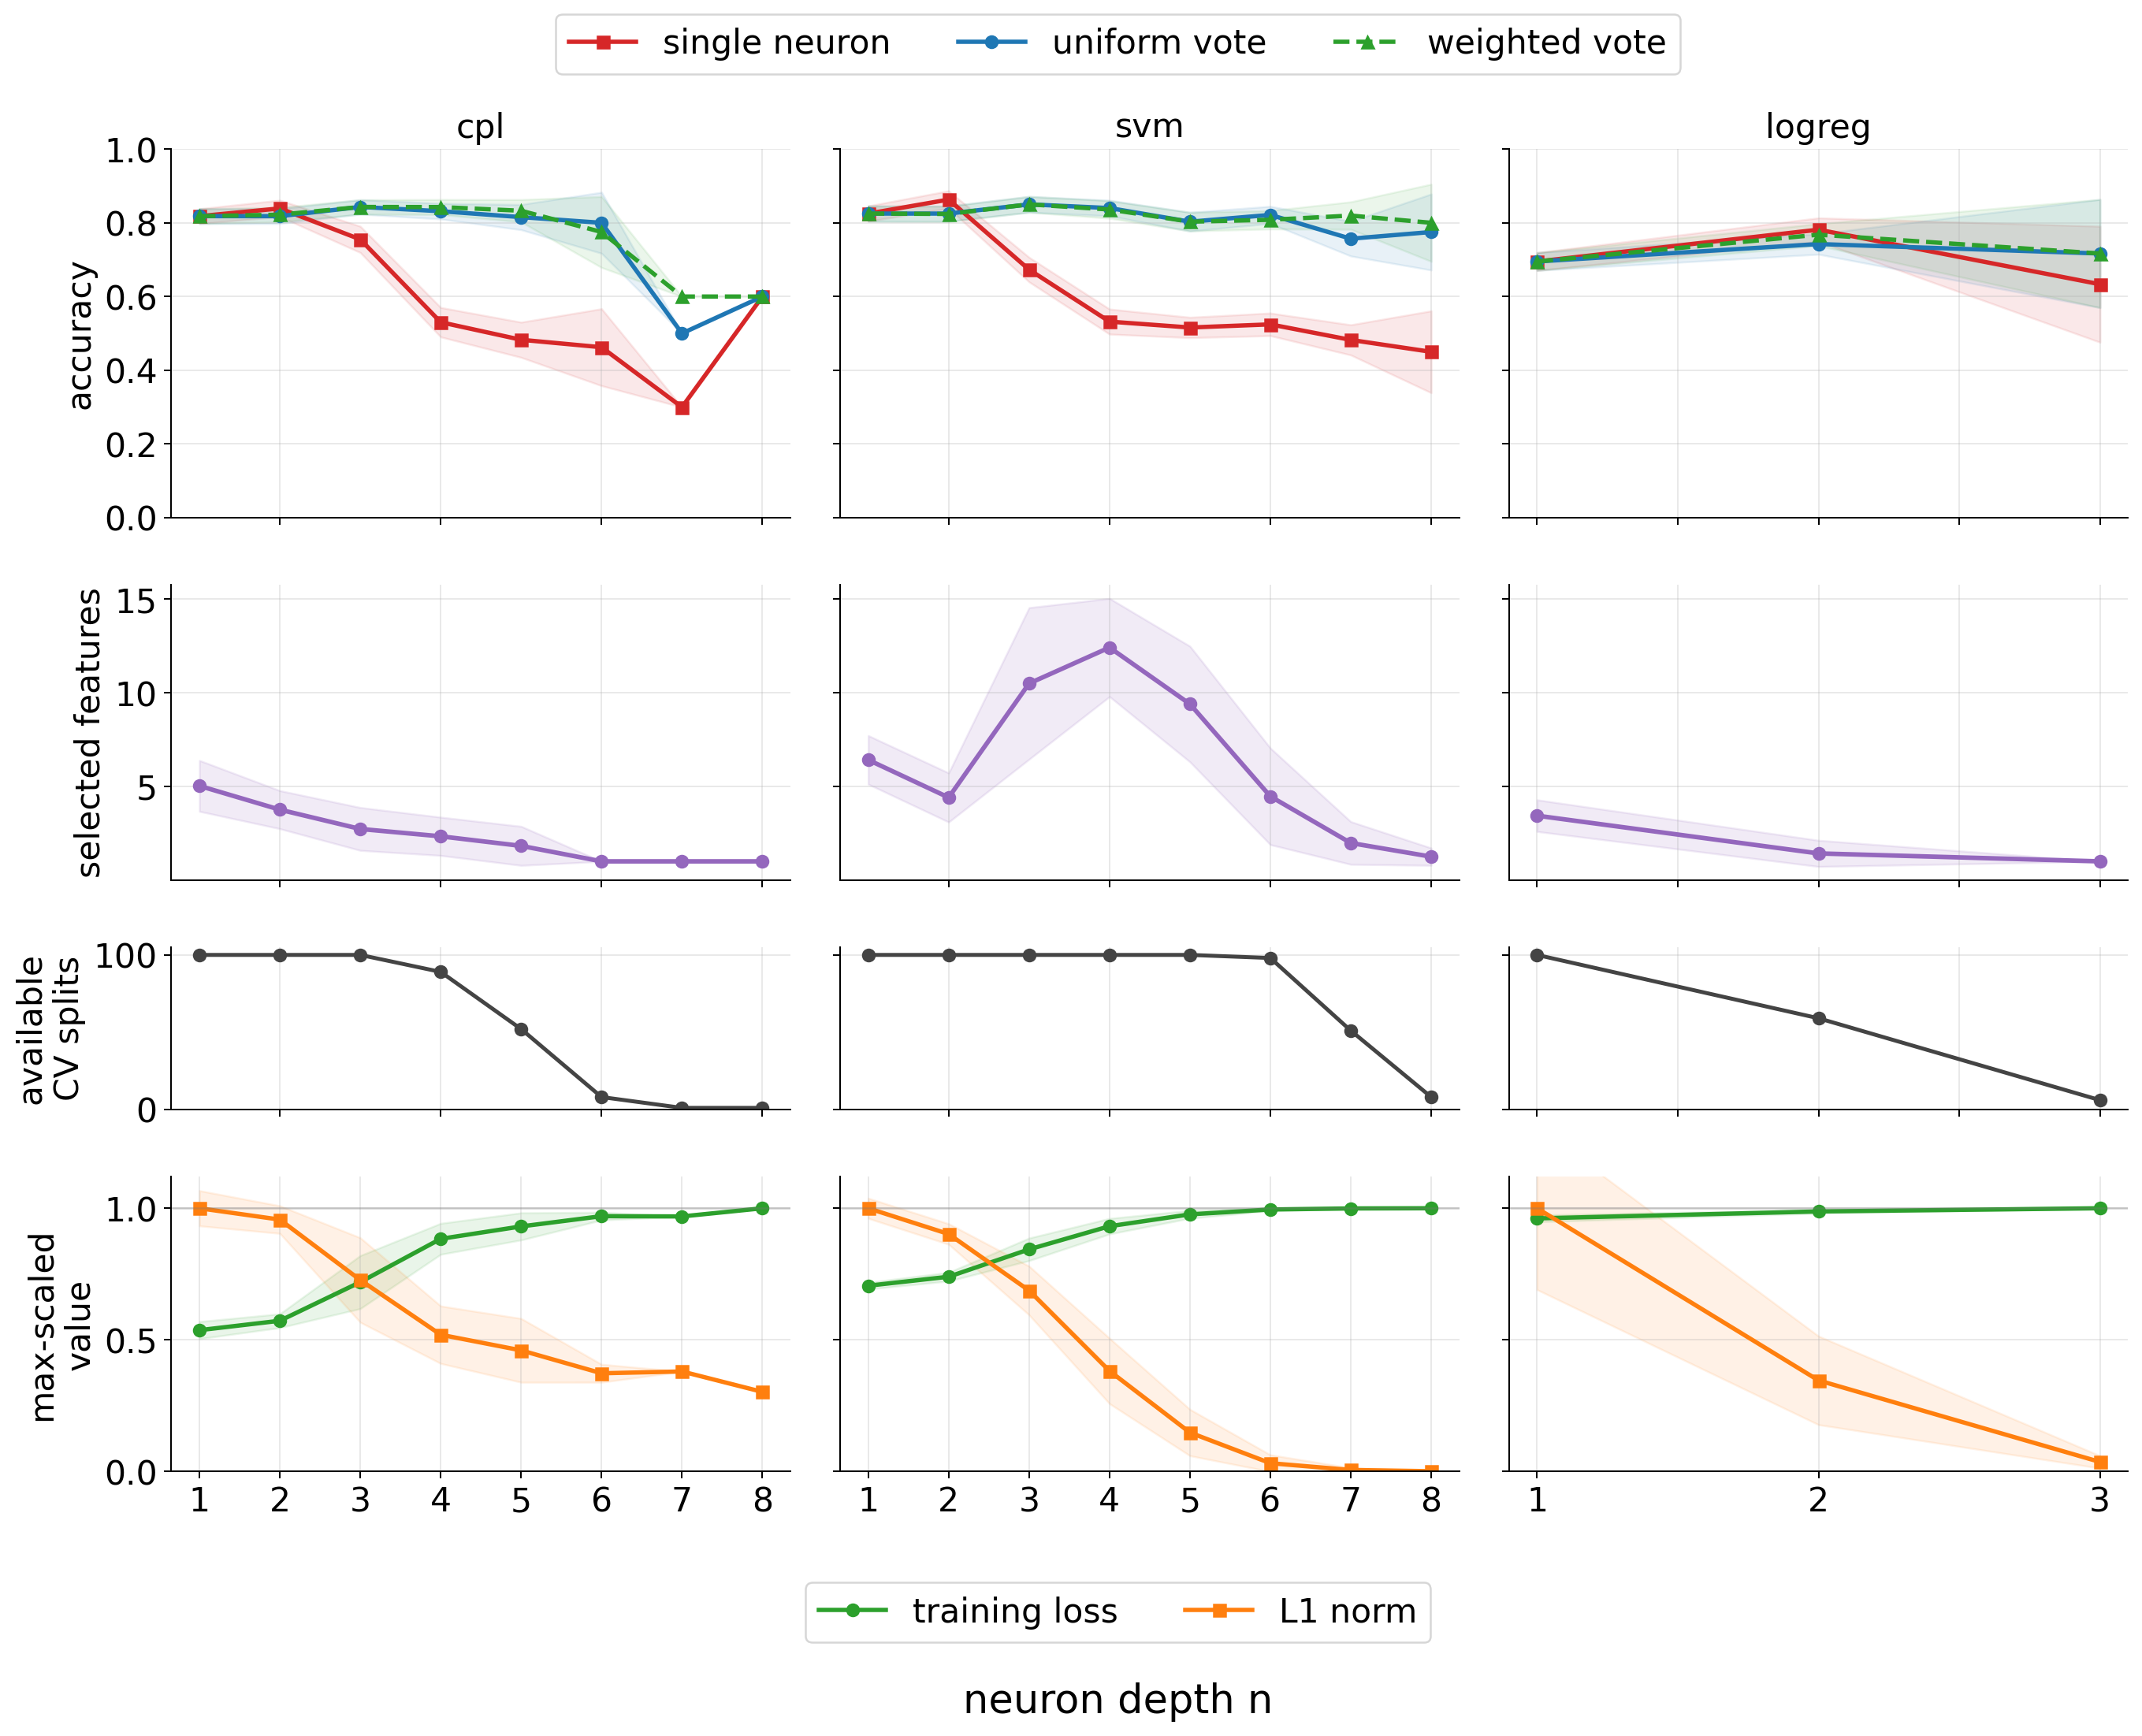
\includegraphics[width=\linewidth]{figures/paper_panels/synthetic_diagnostics_panel.png}
\caption{Low-feature diagnostic trajectories on the synthetic benchmark. Columns show \texttt{cpl},
\texttt{svm}, and \texttt{logreg} with $C_{\mathrm{low}}$. Rows report predictive accuracy, the average number
of features selected by the $n$-th neuron, the number of CV splits in which that neuron depth was available,
and optimization diagnostics for the $n$-th neuron. Training loss and L1 norm are divided by their
within-model maximum values and should be interpreted as shape summaries rather than absolute-scale comparisons.}
\label{fig:synthetic_sparse_accuracy}
\end{figure}

\FloatBarrier

\subsection*{Synthetic feature recovery}
The known informative-feature set in the synthetic benchmark makes it possible to ask whether predictive gains
come from recovering true signal or from selecting broader sets of noisy features.

\begin{table}[ht]
\centering
\small
\setlength{\tabcolsep}{4pt}
\begin{tabular}{llrr@{\hspace{1.8em}}rrr}
\toprule
Model & Regime & \multicolumn{2}{c@{\hspace{1.8em}}}{$n=1$} & \multicolumn{3}{c}{Cumulative at Best $n$} \\
\cmidrule(lr){3-4}\cmidrule(lr){5-7}
 & & Precision & Recall & $n$ & Precision & Recall \\
\midrule
\texttt{cpl} & $C_{\mathrm{low}}$ & 0.6497 & 0.2617 & 3 & 0.6923 & 0.6475 \\
\texttt{svm} & $C_{\mathrm{low}}$ & 0.6425 & 0.3367 & 3 & 0.4114 & 0.6908 \\
\texttt{logreg} & $C_{\mathrm{low}}$ & 1.0000 & 0.2867 & 2 & 1.0000 & 0.3686 \\
\midrule
\texttt{cpl} & $C_{\mathrm{high}}$ & 0.1880 & 0.4033 & 3 & 0.1413 & 0.7767 \\
\texttt{svm} & $C_{\mathrm{high}}$ & 0.2040 & 0.4267 & 4 & 0.0788 & 0.9167 \\
\texttt{logreg} & $C_{\mathrm{high}}$ & 0.3167 & 0.7217 & 1 & 0.3167 & 0.7217 \\
\bottomrule
\end{tabular}
\caption{Informative-feature recovery on the synthetic benchmark. The $n=1$ columns report precision and recall
for the first neuron alone. The cumulative columns are computed over all features selected up to the
best-accuracy depth reported in Table~\ref{tab:synthetic_performance}.}
\label{tab:synthetic_recovery_summary}
\end{table}

These recovery summaries separate two modes of behavior.
Some models, especially high-feature \texttt{logreg}, concentrate much of the ground-truth signal in the first
neuron. Other configurations, including low-feature \texttt{cpl} and \texttt{svm}, recover informative structure
more gradually across successive neurons before later neurons become dominated by noise features.

\begin{figure}[!htbp]
\centering
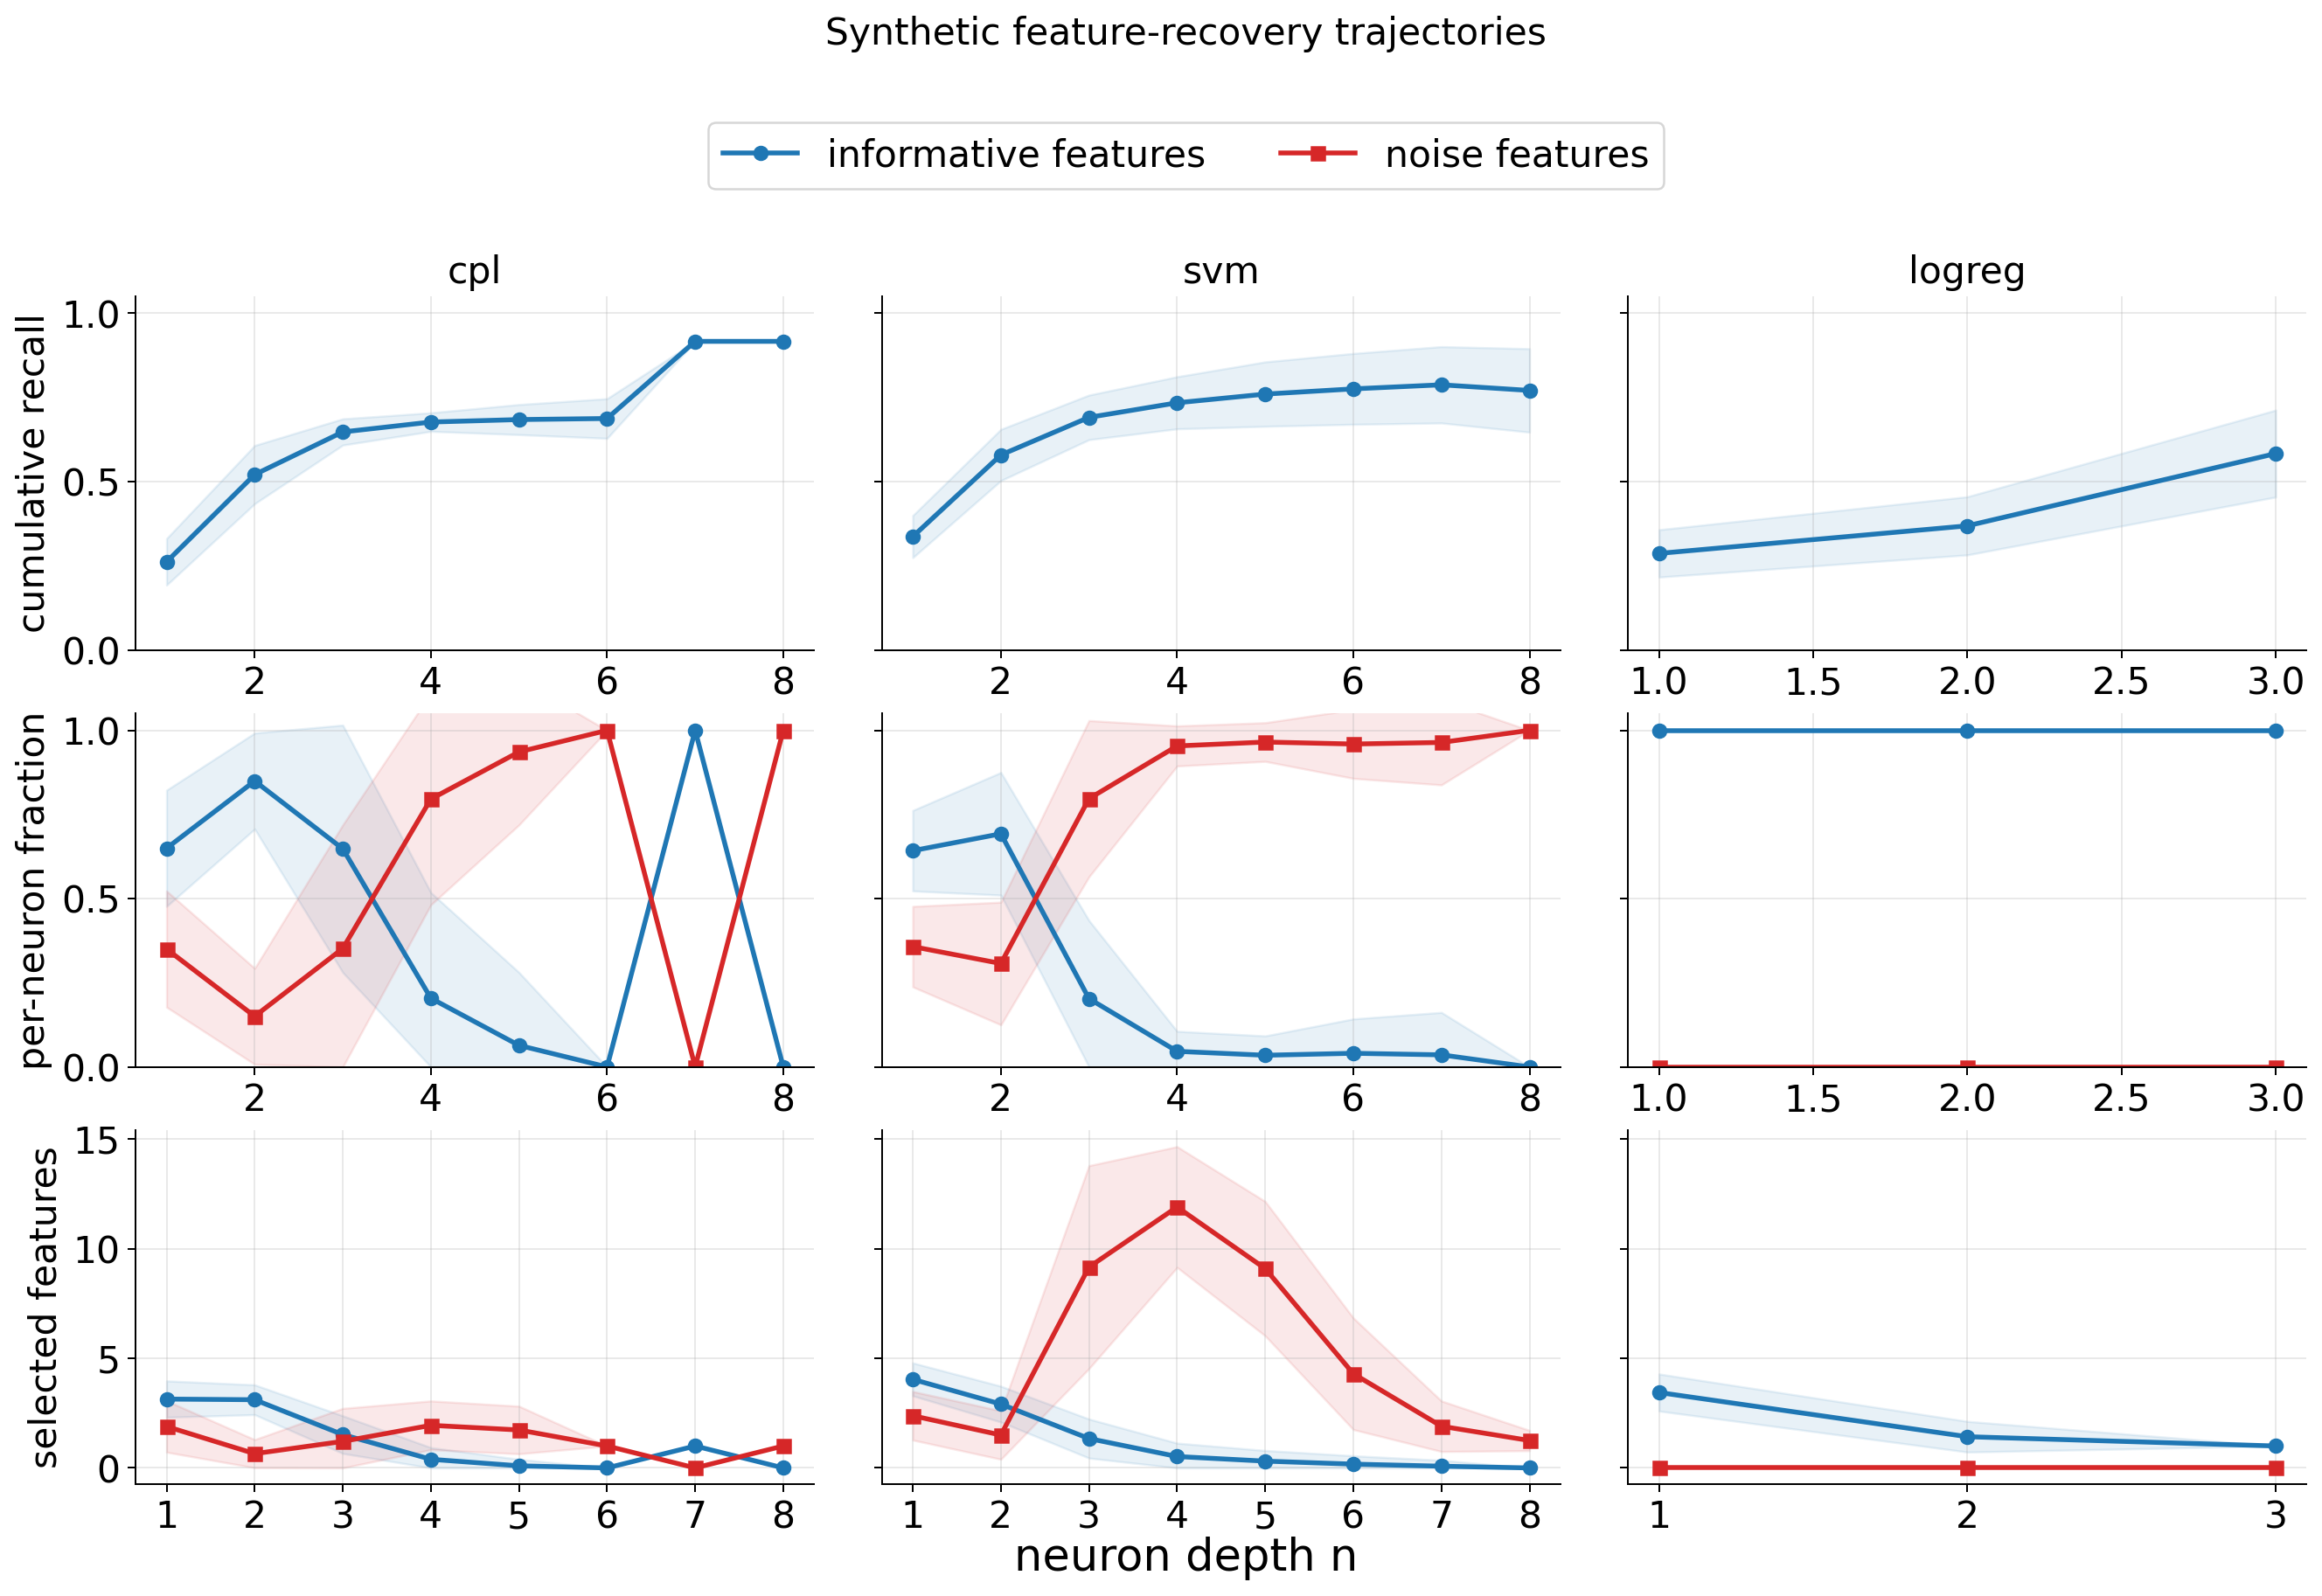
\includegraphics[width=\linewidth]{figures/paper_panels/synthetic_recovery_panel.png}
\caption{Feature-recovery trajectories for the low-feature synthetic benchmark. Columns show \texttt{cpl},
\texttt{svm}, and \texttt{logreg} with $C_{\mathrm{low}}$; rows report cumulative informative-feature recall,
per-neuron informative and noise fractions, and the numbers of informative and noise features selected by the
$n$-th neuron. Blue trajectories describe informative features and red trajectories describe noise features.}
\label{fig:synthetic_sparse_recovery}
\end{figure}

\FloatBarrier

\subsection*{Built depth as a model property}
The nominal maximum depth was 31 neurons, but the realized depth depended strongly on the learner and
regularization.
On the colon cancer benchmark, the realized depth ranged from 3 neurons for low-feature \texttt{logreg} to 31 neurons
for high-feature \texttt{cpl} and high-feature \texttt{svm}.
On the synthetic benchmark, realized depth was markedly smaller, ranging from 3 neurons for low-feature
\texttt{logreg} to 13 neurons for high-feature \texttt{svm}.
This supports the view that neuron depth is not only a reporting axis but also an empirical signature of how
aggressively each base learner exhausts the remaining feature space.
